\begin{figure}

\begin{minipage}{0.16\linewidth}
~
\end{minipage}%
\begin{minipage}{0.42\linewidth}
\centering
Early (Stint $\leq50$)
\end{minipage}%
\begin{minipage}{0.42\linewidth}
\centering
Late (Stint $>50$)
\end{minipage}

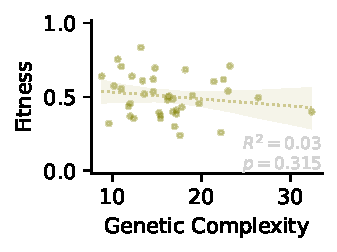
\includegraphics[height=3.5cm,trim={0 1.2cm 0 0},clip]{binder-2025-12-10-complexty-fitness-correlation.ipynb/binder/teeplots/2025-12-10-complexty-fitness-correlation/agg=True+viz=lmplot+when=early+x=genetic-complexity+y=focal-prevalence+ext=.pdf}
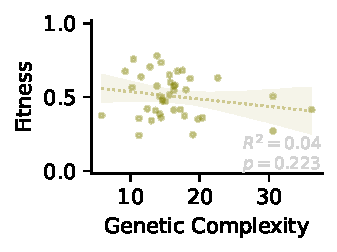
\includegraphics[height=3.5cm,trim={1.7cm 1.2cm 0 0},clip]{binder-2025-12-10-complexty-fitness-correlation.ipynb/binder/teeplots/2025-12-10-complexty-fitness-correlation/agg=True+viz=lmplot+when=late+x=genetic-complexity+y=focal-prevalence+ext=.pdf}



\includegraphics[height=4.4cm,trim={-0.22cm 0 0 0},clip]{binder-2025-12-10-complexty-fitness-correlation.ipynb/binder/teeplots/2025-12-10-complexty-fitness-correlation/viz=lmplot+when=early+x=genetic-complexity+y=focal-prevalence-difference+ext=.pdf}

\includegraphics[height=4.4cm,trim={1.45cm 0 0 0},clip]{binder-2025-12-10-complexty-fitness-correlation.ipynb/binder/teeplots/2025-12-10-complexty-fitness-correlation/viz=lmplot+when=late+x=genetic-complexity+y=focal-prevalence-difference+ext=.pdf}

\caption{
\textbf{Self adaptation drives early complexity.}
\footnotesize
Given the strong association between self adaptation and complexity observed in the case study strain, we sought to assess whether this pattern generalized across replicates.
For this purpose, we measured fitness of sample genomes drawn from each replicate at 10-stint intervals --- taken as the fraction of competition trials won against cross-replicate comparators, using a biotic background design to incorporate context effects (Figure \ref{fig:fit:bbg}).
Self adaptation could then be calculated as the difference between fitness in self context versus co-evolved context.
Across early stints ($\leq50$), we found a robust positive association between self adaptation and genetic complexity (bottom left; $p < 10^{-5}$, $R^2 = 0.41$, two-tailed Wald test).
Beyond this point, however, association between genetic complexity and self adaptation dissipated (bottom right).
Surpringly, no correlation arose between genetic complexity and fitness (top row).
Here, fitness was measured against cross-replicate comparators using 50/50 competition trials (Figure \ref{fig:fit:nobbg}).
}
\label{fig:fit-advantage-correlations}

\end{figure}
